\section{Benchmarking}
\label{sec:res_bench}
This section presents the result from the IOZone benchmarking tests run on each filesystem. The output result is divided into a table for each test for each filesystem. Each table presents the benchmark performance of the test for each file size and each buffer size.Each table has five rows and 13 columns, where each cell is the performance of the test with the specific file size and buffer size. The complete data tables and graphs presenting the performance of each file system for the different file sizes can be found in Appendix~\ref{app:bench_data}.

The IOZone benchmarking for \gls{FFS} ran for 41 minutes, and the IOZone benchmarking for \gls{GCSF} took 20 minutes. They were started at the same time and the internet speed tests ran every five minutes until the benchmarking of \gls{FFS} was completed. In total, eight speed tests were conducted with an average latency of \SI{15.22}{\milli\second}. The average download speed was \SI[per-mode = symbol]{90.96}{\mega\bit\per\second} and the average upload speed was \SI[per-mode = symbol]{92.95}{\mega\bit\per\second}.

Combining the 55 data points in one table, we get the overall performance of a test. Using this data, we can plot a box plot presenting the spread of the values in the table. Figure~\ref{fig:res_box_ffs} presents a box plot of the benchmarking results of \gls{FFS}. It can be observed that the Read, \mbox{Re-Read}, and Random Read operations are significantly faster than the Write, \mbox{Re-Write}, and Random Write operations. The Write, \mbox{Re-Write}, and Random Write operations all have a wide spread of values. It can also be noted that the median performance of \mbox{Re-Read} and Random Read are better than the median performance of Read. The median performance of \mbox{Re-Read} and Random Read are comparable where Random Read has a bigger spread of values.

Figure~\ref{fig:res_box_gcsf} presents a box plot of the benchmarking results of \gls{GCSF}. It shows that Write, \mbox{Re-Write}, and Random Write have significantly less performance than the results of Read, \mbox{Re-Read}, and Random Read. It can be noted that the median performance of \mbox{Re-Write} and Random Write are similar, and both are less than the median performance of Write. The median performance of \mbox{Re-Read} and Random Read are higher than the median performance of Read.

Figure~\ref{fig:res_box_fffs} presents a box plot of the benchmarking results of \gls{FFFS}. In this plot, one can see that the spread of the values from Write and \mbox{Re-Write} is high. Looking at Table~\ref{tbl:data_write_fejk_ffs}, we can see that certain values are indeed greater than the most, such as \texttt{file size = 2048, buffer size = 128} where the performance is \SI[per-mode = symbol]{116330}{\kilo\byte\per\second} which is significantly more than most values in the table. Further, Figure~\ref{fig:res_box_fffs} shows that Read, \mbox{Re-Read} and Random Read have similar performances, where the median and best performance of \mbox{Re-Read} and Random Read is better than the median and best performance of Read. Random Write has less of a spread than Write and \mbox{Re-Write} has, and the median performance of Random Write is better than the median performance of both Write and \mbox{Re-Write}.

Figure~\ref{fig:res_box_apfs} presents a box plot for \gls{APFS}. In this figure, it is possible to see that the performance of the different write operations is lower than the performance of the read operations. Further, it can be noted that the median performance of the \mbox{Re-Read} and the \mbox{Re-Write} tests is better than the performance of the standard Read and Write tests. The median performance of Random Read is similar to the median performance of Read, but the median performance of Random Write is significantly lower than the median performance of Write.

\begin{figure}[!htb]
	\label{fig:res_box_ffs}
	\begin{center}
		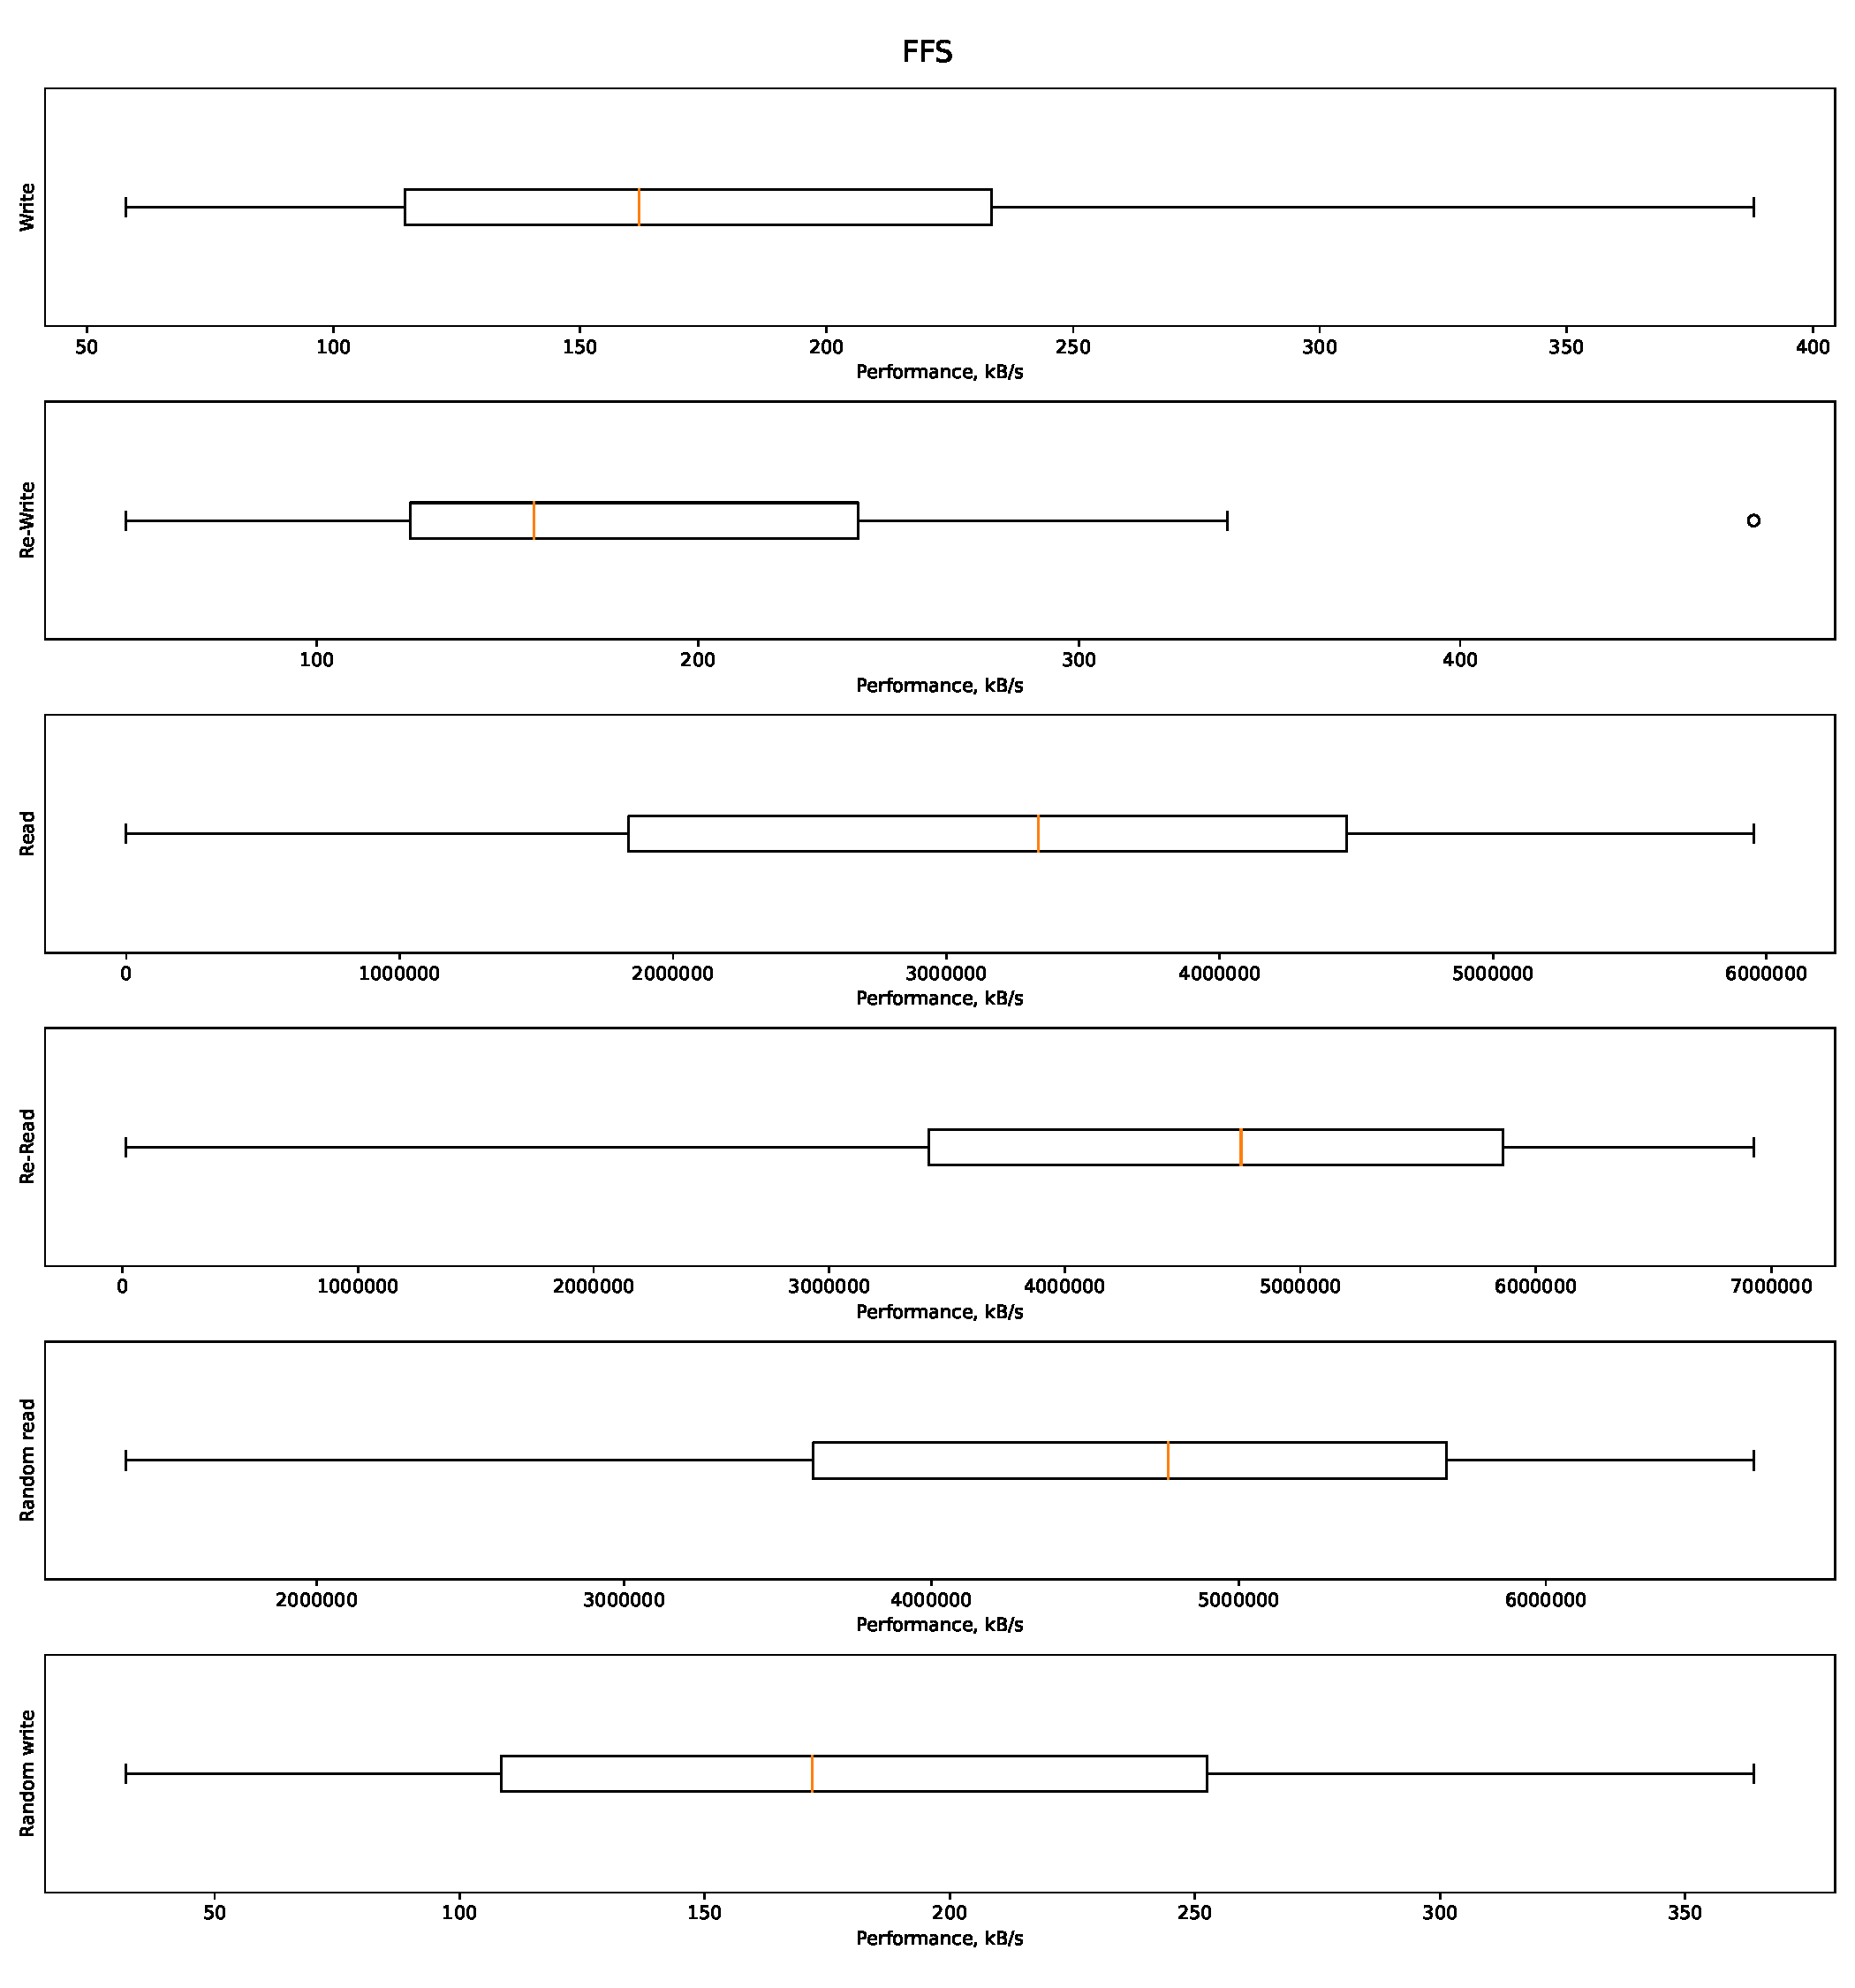
\includegraphics[width=1.0\textwidth]{figures/benchmarking/ffs/FFS-box.pdf}
	\end{center}
	\caption{Box plot of the IOZone output for the different tests for \gls{FFS}}
\end{figure}

\begin{figure}[!htb]
	\label{fig:res_box_gcsf}
	\begin{center}
		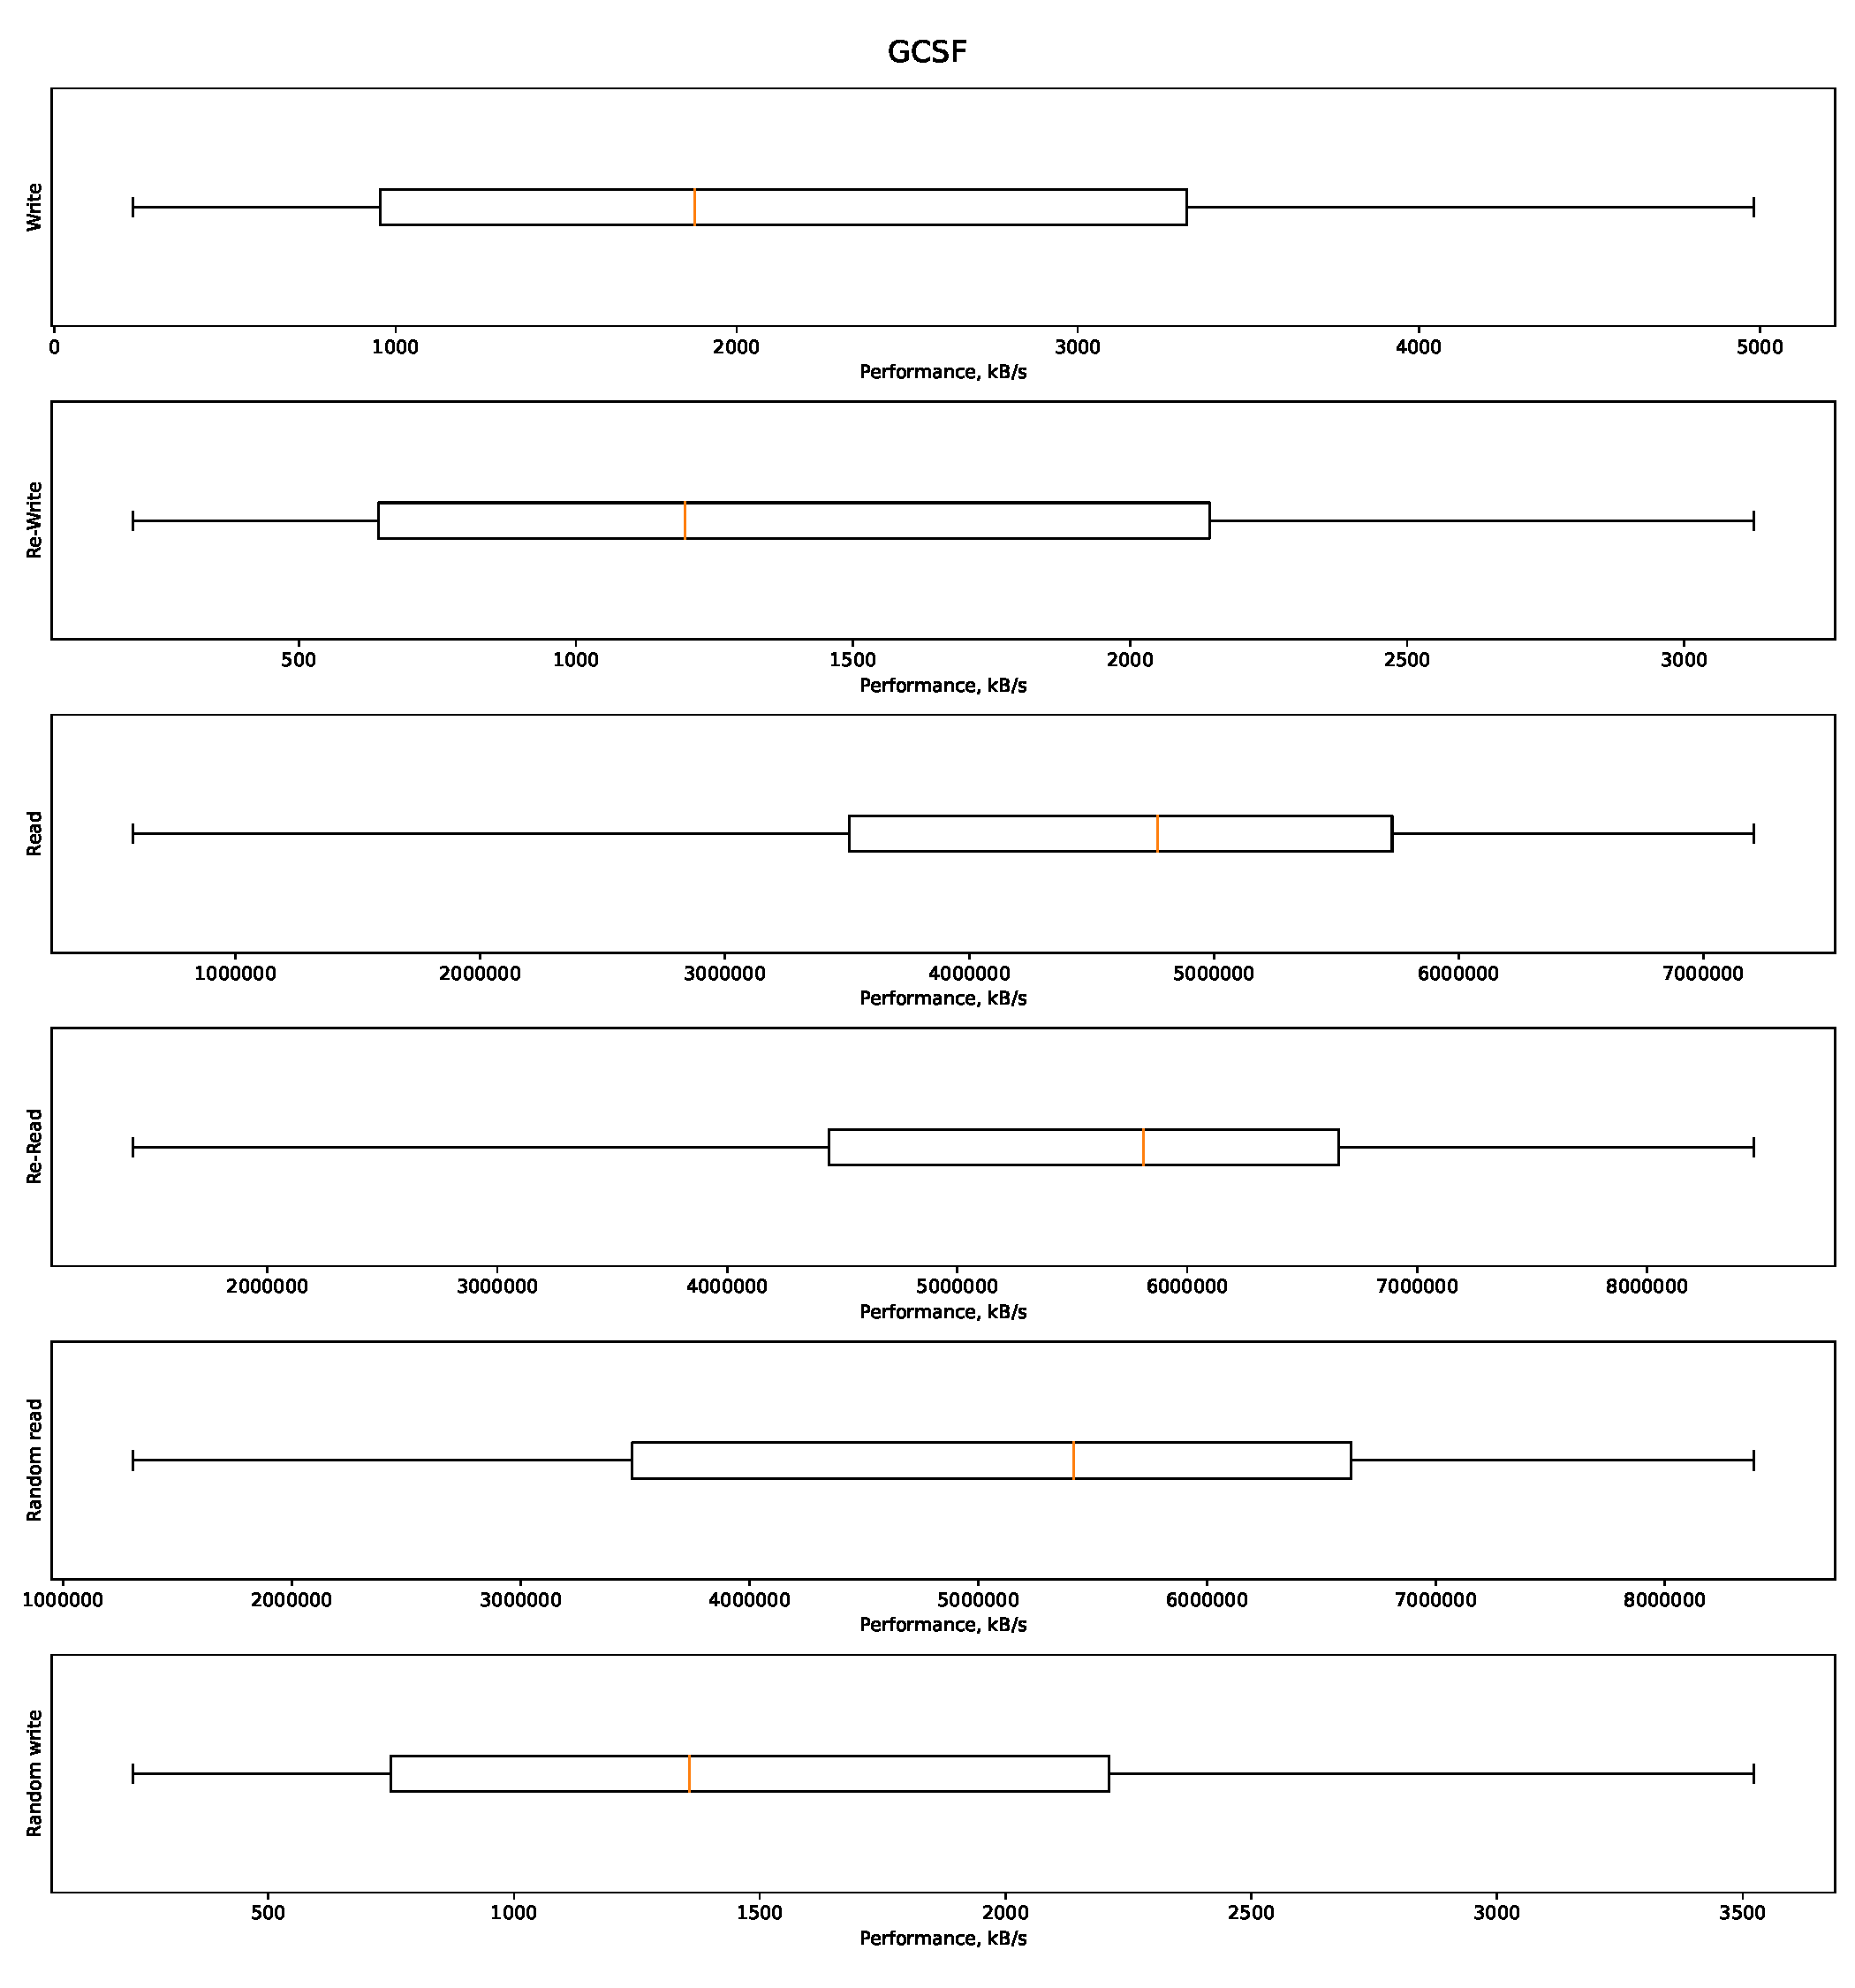
\includegraphics[width=1.0\textwidth]{figures/benchmarking/gcsf/GCSF-box.pdf}
	\end{center}
	\caption{Box plot of the IOZone output for the different tests for \gls{GCSF}}
\end{figure}

\begin{figure}[!htb]
	\label{fig:res_box_fffs}
	\begin{center}
		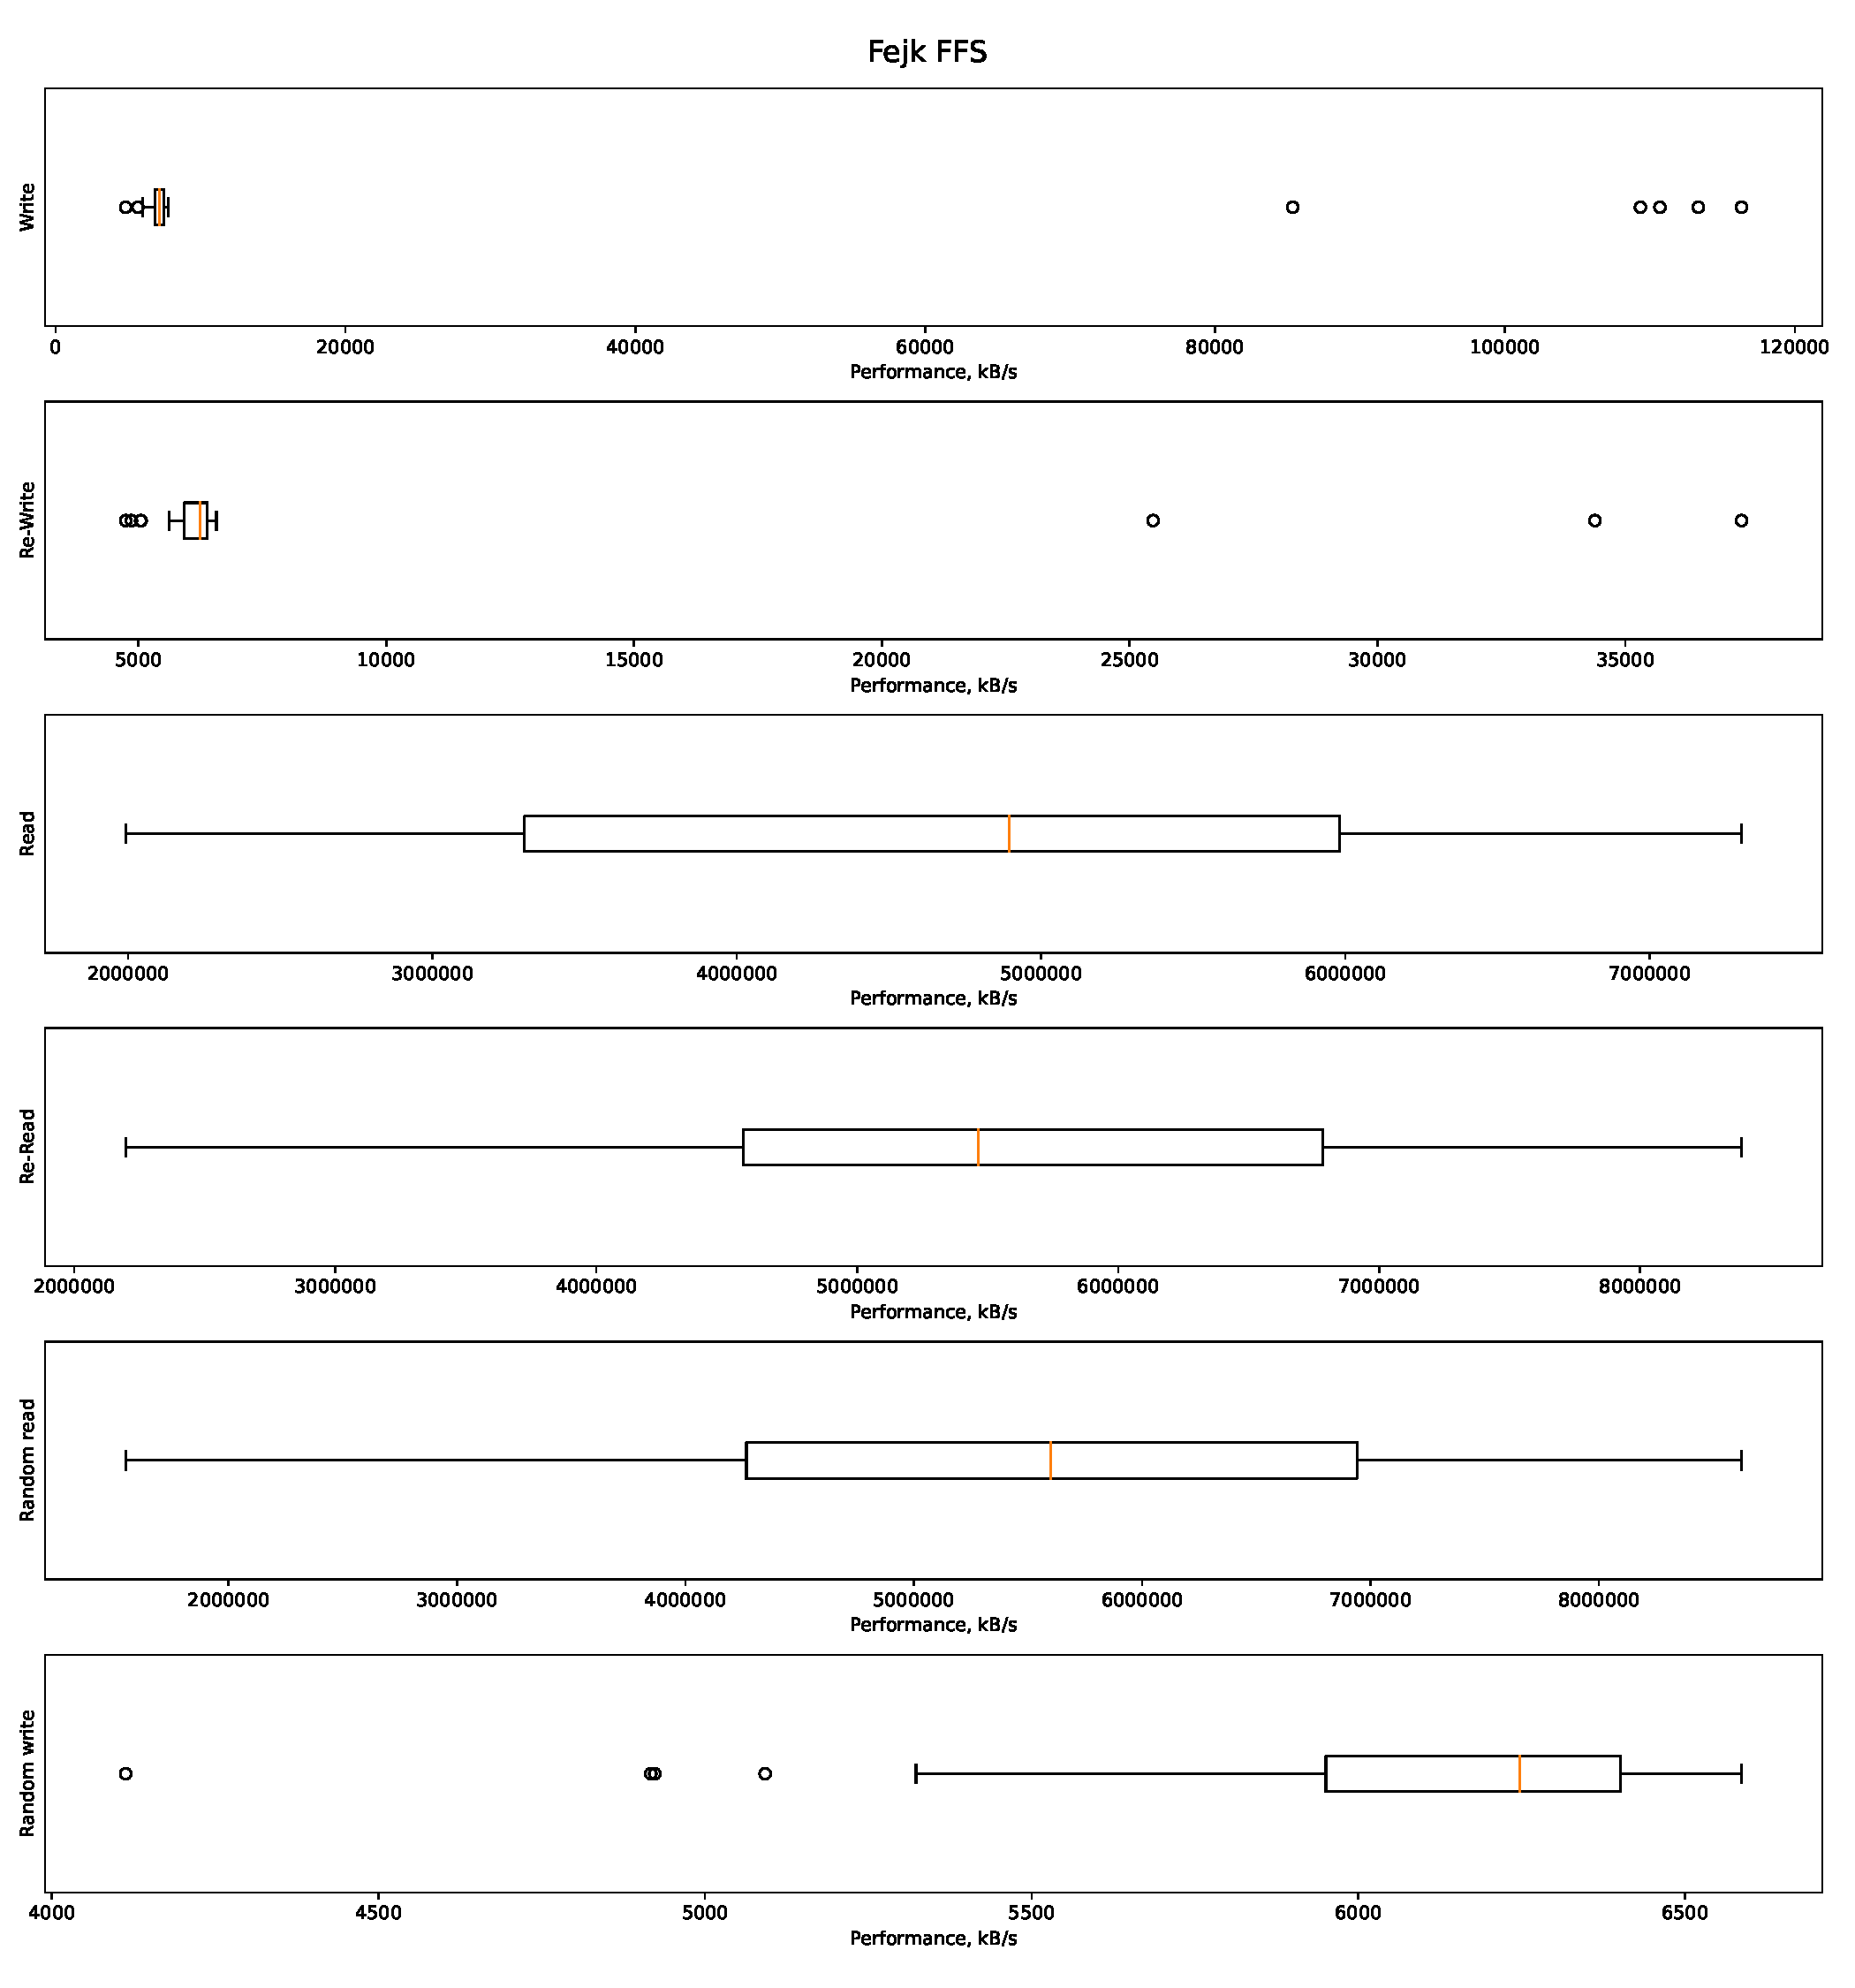
\includegraphics[width=1.0\textwidth]{figures/benchmarking/fake-ffs/Fejk FFS-box.pdf}
	\end{center}
	\caption{Box plot of the IOZone output for the different tests for \gls{FFFS}}
\end{figure}

\begin{figure}[!htb]
	\label{fig:res_box_apfs}
	\begin{center}
		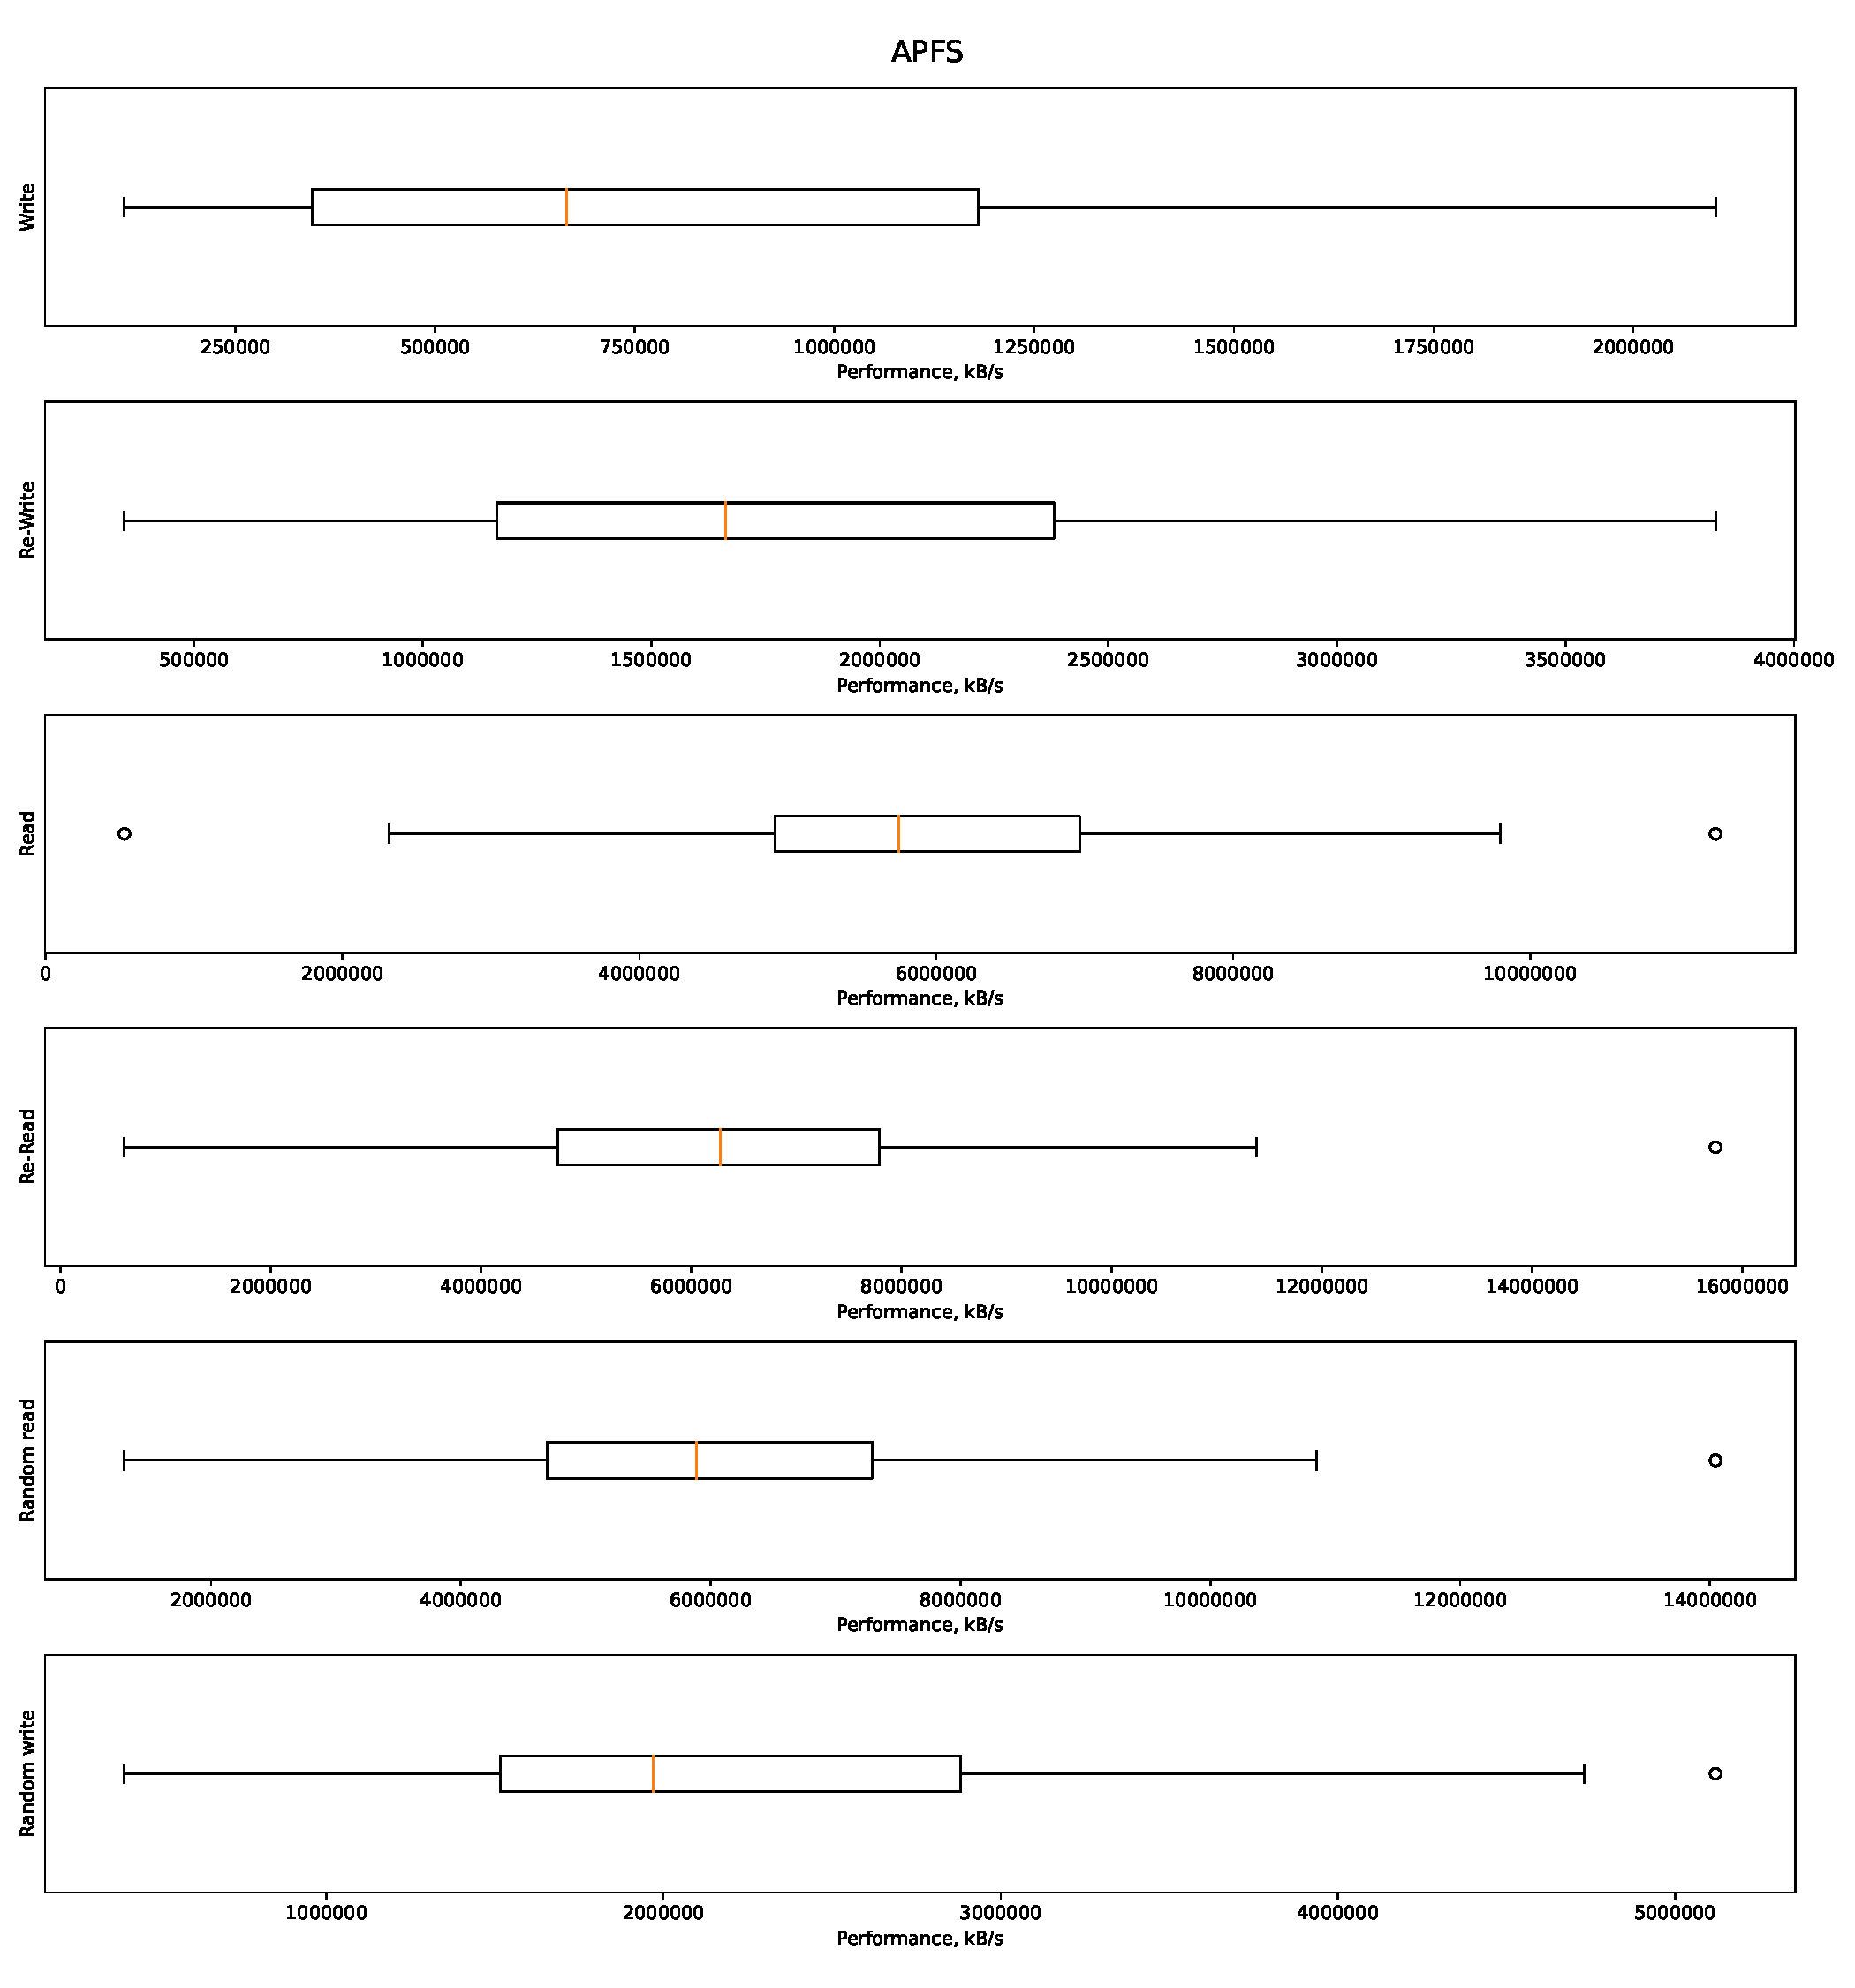
\includegraphics[width=1.0\textwidth]{figures/benchmarking/local/APFS-box.pdf}
	\end{center}
	\caption{Box plot of the IOZone output for the different tests for \gls{APFS}}
\end{figure}